\chapter{Implications}
\label{chap:implications}


\section{Internal and External Perspectives}

What we observe is that we are a small subset $O$ of  the huge superset $U$.

% ============================================================
% DIAGRAM 1: Intuitive Dualism (O \subset U)
% ============================================================
\begin{figure}[htbp]
\centering
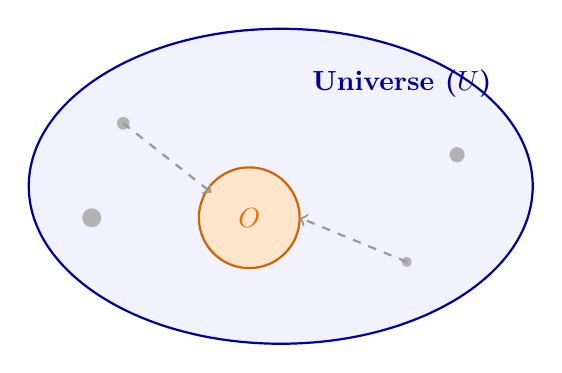
\begin{tikzpicture}[scale=0.8]
    % Large external Universe
    \draw[thick, fill=blue!5, draw=blue!60!black] (0,0) ellipse (4cm and 2.5cm);
    \node[anchor=north east, blue!60!black] at (3.5, 2) {\textbf{Universe ($U$)}};
    
    % Tiny distant stars/structures in U
    \fill[gray!60] (-2.5,1) circle (0.1);
    \fill[gray!60] (-3,-0.5) circle (0.15);
    \fill[gray!60] (2,-1.2) circle (0.08);
    \fill[gray!60] (2.8,0.5) circle (0.12);
    
    % Small Observer contained inside
    \draw[thick, fill=orange!20, draw=orange!80!black] (-0.5,-0.5) circle (0.8cm);
    \node[orange!90!black] at (-0.5,-0.5) {\textbf{$O$}};
    
    % Incoming "signals" (Naive representation)
    \draw[->, dashed, thick, gray!80] (2, -1.2) -- (0.3, -0.5);
    \draw[->, dashed, thick, gray!80] (-2.5, 1) -- (-1.1, -0.1);
\end{tikzpicture}
\caption{\textbf{The Initial Observational Relation ($O \subset U$).} A conceptual diagram illustrating the baseline standard view of naive realism. The finite observer ($O$) is modeled as a small physical subset contained entirely within, and fundamentally dwarfed by, an immense, independent, external Universe ($U$). Information is assumed to transmit across a boundary from outside to inside.}
\label{fig:diag1}
\end{figure}

\newpage

However, if the axioms hold, we have to accept the fact that this is
only our internal perspective. In static universe no metaphysical
signals flip bits inside us because other bits fipped far away.
All dynamics, time, information we receive through our eys and senses
must already be present in us. Therefore, we are not sub-set
of the universe, it must be the other way around. The universe is in us. 


% ============================================================
% DIAGRAM 2: The Inversion of Containment (U \subset O)
% ============================================================
\begin{figure}[htbp]
\centering
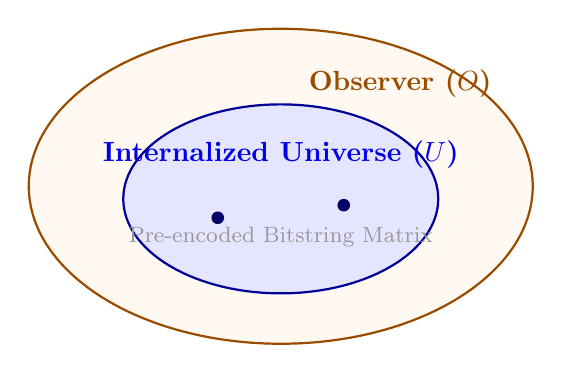
\begin{tikzpicture}[scale=0.8]
    % Large Observer acting as the boundary
    \draw[thick, fill=orange!5, draw=orange!60!black] (0,0) ellipse (4cm and 2.5cm);
    \node[anchor=north east, orange!60!black] at (3.5, 2) {\textbf{Observer ($O$)}};
    
    % Internalized Universe completely inside the observer
    \draw[thick, fill=blue!10, draw=blue!60!black] (0,-0.2) ellipse (2.5cm and 1.5cm);
    \node[blue!90!black] at (0, 0.5) {\textbf{Internalized Universe ($U$)}};
    
    % Features of the universe are now features of the observer's code
    \fill[blue!40!black] (-1,-0.5) circle (0.1);
    \fill[blue!40!black] (1,-0.3) circle (0.1);
    \node[gray!80, font=\footnotesize] at (0, -0.8) [font=\footnotesize] {Pre-encoded Bitstring Matrix};
\end{tikzpicture}
\caption{\textbf{The Inversion of Containment ($U \subset O$).} A topological inversion forced by the IEP axioms. Because no metaphysical signals can cross from a non-existent external reality into a static bitstring, any universe experienced by the observer must be entirely contained *within* the structural limits of the observer's own informational state.}
\label{fig:diag2}
\end{figure}

\newpage

The both perspectives, internal and external, are undeniable. The
only solution that allows this is that the both sets $O$ and $U$
are the same set. 


% ============================================================
% DIAGRAM 3: The Structural Identity Solution (O = U)
% ============================================================
\begin{figure}[htbp]
\centering
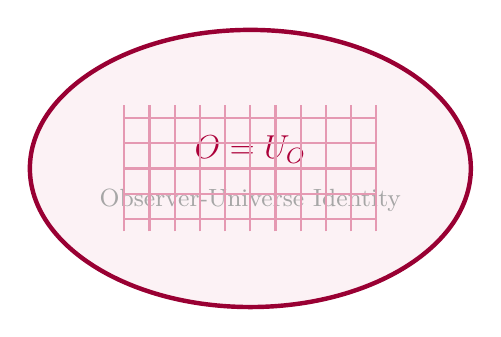
\begin{tikzpicture}[scale=0.8]
    % A single, unified boundary where O and U are co-extensive
    \draw[ultra thick, fill=purple!5, draw=purple!80!black] (0,0) ellipse (3.5cm and 2.2cm);
    
    % Labels pointing to the same space
    \node[purple!90!black, font=\large] at (0,0.3) {\textbf{$O = U_O$}};
    \node[gray!70, font=\small] at (0,-0.5) {Observer-Universe Identity};
    
    % Internal structural complexity representing both physical laws and conscious state
    \draw[thick, color=purple!40, step=0.4cm] (-2,-1) grid (2,1);
\end{tikzpicture}
\caption{\textbf{The Structural Identity Solution ($O = U$).} The final single-observer synthesis. To resolve the contradiction between empirical observation ($O \subset U$) and informational closure ($U \subset O$), the boundaries are collapsed. The observer and their experienced universe are identical, unified aspects of a single, static information topology.}
\label{fig:diag3}
\end{figure}

\newpage

We also observer other observers. And due to the probabilistic nature
of the theory, it would be extremely difficult to argue that only one
observer is allowed. And because of the effectiveness of mathematics,
the only logical conclusion is that the universe is the intersection
of the observers.

Reality is observer relative. 


% ============================================================
% DIAGRAM 4: The Multi-Observer Intersubjective Reality
% ============================================================
\begin{figure}[htbp]
\centering
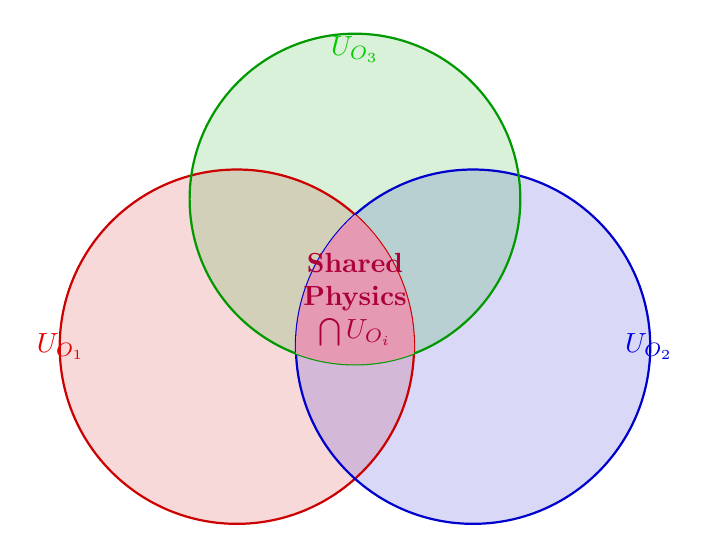
\begin{tikzpicture}[scale=0.75]
    % Scope for opacity mixing
    \begin{scope}[fill opacity=0.15]
        % Observer 1
        \fill[red!80!black] (-2,0) circle (3cm);
        % Observer 2
        \fill[blue!80!black] (2,0) circle (3cm);
        % Observer 3
        \fill[green!60!black] (0,2.5) circle (2.8cm);
    \end{scope}
    
    % Outlines
    \draw[thick, red!80!black] (-2,0) circle (3cm) node[left=1.8cm, red!90!black] {\textbf{$U_{O_1}$}};
    \draw[thick, blue!80!black] (2,0) circle (3cm) node[right=1.8cm, blue!90!black] {\textbf{$U_{O_2}$}};
    \draw[thick, green!60!black] (0,2.5) circle (2.8cm) node[above=1.6cm, green!80!black] {\textbf{$U_{O_3}$}};
    
    % Central Shared Intersection
    \begin{scope}
        \clip (-2,0) circle (3cm);
        \clip (2,0) circle (3cm);
        \clip (0,2.5) circle (2.8cm);
        \fill[purple!40] (0,0) circle (5cm); % highlights the intersection
    \end{scope}
    
    % Label for Objective Reality
    \node[purple!90!black, font=\bfseries, text width=2.5cm, align=center] at (0,0.8) {Shared\\Physics\\$\bigcap U_{O_i}$};
    
\end{tikzpicture}
\caption{\textbf{The Multi-Observer Intersubjective Reality.} Escaping solipsism via intersection. Objective reality is not an independent "container room" that observers inhabit. Instead, what we call objective physical reality is the shared structural intersection ($\bigcap U_{O_i}$) of invariant, highly compressible information common to independent observer bitstrings.}
\label{fig:diag4}
\end{figure}


This leads to the prediction, that part of observers structure is
fundamentally inaccessible to other observers. 

We will never be able to reduce the operation of Alice to
neurons in her brain, because observable Alice is just vanishingly
small slice of total information compricing her. 


\section{The Unreasonable Effectiveness of Mathematics}

In standard physicalism, the Wigner's "unreasonable effectiveness"  \cite{wigner1960} is a mystery because we assume there is a
physical world made of "stuff" out there, and for some bizarre reason,
human abstract thoughts (math) mirror its behavior perfectly.

In this framework, this is completely inverted: There is no external "stuff." There are only bitstrings—pure combinatorics and mathematical relations.

The Intersection Minimizes Description Length: The shared universe ($U_{\text{share}} = \bigcap U_{O_i}$) isn't an arbitrary room; it is the specific subset of highly compressible, invariant data common to independent observer bitstrings.

For minimal description length multiple observers must be made of common sub-structures.

Therefore, mathematics isn't an accidental tool that happens to describe a separate physical world.
Mathematics is the very fabric of the intersection itself.

Observers don't just happen to find themselves in universes with identical mathematical laws by luck.
They share the same mathematics because any structure capable of being shared and compressed among independent observers is,
by definition, mathematical.

If a piece of information couldn't be compressed or governed by an invariant rule (a mathematical law),
it couldn't survive the intersection filter to become part of intersubjective, verifiable physics.
It would remain part of the private, inaccessible structure unique to an individual observer.

The "effectiveness" isn't a miraculous coincidence; it is a strict structural requirement for the existence of a shared reality.


\section{Is the Universe Fundamentally Continuous or Discrete?}

To anchor this question into plain intuition, we can utilize a pedagogical thought experiment.
Imagine an intelligent observer---say, a liquid-metal Terminator T-1000 ---living inside a high-fidelity, computer-generated movie.
We chosen T-1000 not because its superiority as a violent killing machine, but because it's
perfectly smooth continuous surface.

This universe is rendered frame-by-frame as a 3D video composed of discrete voxels (volumetric 3D pixels).
To keep the storage file size manageable, the creators use a sophisticated, complex-valued 3D-QMPEG compression codec.

On a macroscopic scale, the T-1000 perceives its world as a smooth, continuous geometric manifold.
Everything at this scale appears as perfectly continuous surfaces,
modeled with parametric Non-Uniform Rational B-Splines (NURBS) of a high mathematical degree, defined within a Lorentzian signature.
The T-1000 navigates this geometric theater flawlessly using the intuitive laws of smooth motion.

Then, the T-1000 decides to become a physicist.
As it begins to zoom in and probe the absolute limits of its reality, it makes a series of startling discoveries:
\begin{itemize}
    \item \textbf{The Artifact of Compression:} It notices that its seemingly continuous skin is actually composed of discrete, bounded voxels.
    \item \textbf{The Spectral Signature:} It finds that these voxels do not update or change positions randomly.
      Instead, their coordinates and densities are governed by interference patterns, phases, and frequency coefficients.
    \item \textbf{The Discovery of Quantum Mechanics:} The T-1000 has just ``discovered'' Quantum Mechanics.
      It realizes that to accurately model the state of any single voxel, it must use a complex-valued unitary wavefunction.
\end{itemize}

The T-1000 might naturally ask: \emph{``Why do I live in a world of complex-valued waves (Hilbert space) instead of just smooth shapes (Einsteinian space)?''}
Furthermore, driven by standard reductionist thinking, it might begin developing a monumental $10^{500}$ Voxel String Theory to mathematically smash the macro-continuum of its world into pieces.

But this is a category error.
The T-1000 is simply looking at the compression artifacts of its own reality.
The ``waves'' are not an additional, underlying basement of material complexity; they are the most informationally efficient way to represent and store discrete voxels with minimal code overhead.
Trying to quantize smooth geometry to build a theory of everything is merely attempting to find pixels inside an analytic equation.


\section{The Hollow Simulation Objection}

The most common objection to computational accounts of mind is the hard
problem of consciousness \cite{Chalmers1996}: a simulated human, even if
behaviourally identical to a biological human, might be ``hollow'' --- it
might lack subjective experience while producing identical outward behaviour.

The Proposition in Paper~I directly refutes this
objection within the axiomatic system. By $A_2$, the biological human is a
computable physical system whose state transitions are fully determined by
physical law and initial conditions. By $A_3$, a simulation exists whose
execution trace is isomorphic to that of the biological human, preserving
all causally relevant internal relations. By $A_4$, subjective experience
contributes to observable behaviour. If the simulation lacked subjective
experience while remaining behaviourally identical, subjective experience
would be causally inert, contradicting $A_4$.

The hollow simulation is therefore not merely implausible; it is
inconsistent with the four axioms. Accepting the hollow simulation requires
rejecting at least one axiom.


\section{Entropy Gradients and Observer Self-Location}

The probability of rich, persistent geometric structure is not monotonic in entropy.
Very low entropy lacks sufficient differentiation for stable geometry.
Very high entropy dissolves coherence. Complex, long-lived observers therefore dominate only near intermediate entropy values.

Observers necessarily find themselves on one side of this entropy peak.
Their experienced universe is shaped by this self-location relative to the log-normal shaped probability gradient.

An observer located on the low-entropy side of the peak experiences successive configurations of \emph{increasing} entropy and differentiation.
The perceived universe expands, a singularity appears in the past, and structure emerges irreversibly. This corresponds to what we traditionally call the Big Bang and cosmological expansion.

An observer located on the high-entropy side experiences \emph{decreasing} entropy and tightening constraints.
The perceived universe contracts, a singularity appears in the future, and matter falls inward without escape.
This corresponds to a black hole.

These are not two different objects. They are complementary readings of the \emph{same} timeless informational structure,
interpreted from opposite sides of the probability gradient.
Expansion and collapse are epistemic phenomena induced by the observer’s self-location along the entropy profile.


\section{Observer Mortality}

Observer's wavefunction gets more complex as observers age for various reasons, such as memory.
Initially, this increases the probability of survival by allowing for better reasoning and prediction.

However, as informational complexity increases it sooner or later becomes a liability.
The increasing complexity reduces compressibility; eventually, no high-probability continuations remain.
The observer ceases to exist through vanishing measure.

The geometric projection gradually deteriorates.
Wrinkles appear; highly developed biceps and triceps wither.
Your back hurts. People have to shout for any message to get through.
In no time, you lie in bed, trusting someone to change your diapers.
This is what a higher-frequency information model looks like when projected onto geometric spacetime.
Sooner or later, the induced measure drops below a critical threshold, probabilities dry out, and the observer's time is up.

You have run out of all the configurations describing "you."

Death is therefore a statistical event: the exhaustion of observer-compatible configurations.


\section{Informational Cost of Intelligence}

If the probability of an observer is governed by the minimal description length, 
a natural question arises: what is the role of intelligence?

Consider a classical analogy: a sphere rolling down a potential valley follows the path of least action.
Its trajectory is easy to describe and carries minimal informational cost.

Now suppose the sphere is replaced by an intelligent observer capable of anticipating future outcomes.
It realizes that the minimal-cost path leads to a fatal collision with another observer.
To avoid death, it deliberately chooses a more complex trajectory.

So can the observer, via logical reasoning, actually choose informationally more expensive path now, to avoid dying later? 

Let $\gamma_{\rm passive}$ be the natural minimal-cost path in the absence of intelligence, and $\gamma_{\rm active}$ the path deliberately chosen by the intelligent observer.
We define the \emph{informational cost of intelligence} as
\[
\Delta \mathcal{C}_{\rm int} = \mathcal{C}_O[\gamma_{\rm active}] - \mathcal{C}_O[\gamma_{\rm passive}],
\]
where $\mathcal{C}_O[\gamma]$ is the total spectral-geometric complexity of trajectory $\gamma$.

Sudden death later will inject enormous high-frequency content into the observer's wavefunction, dramatically increasing the description length of total observer path.
Intelligence, by contrast, acts as an internal sensor of future compressibility.
Formally, intelligent behavior selects the trajectory that minimizes the expected future complexity:
\[
\gamma_{\rm active} = \arg\min_\gamma \mathbb{E}\bigl[\mathcal{C}_O[\gamma_{\rm future}]\bigr].
\]

Intelligence is therefore not an extra cost, but a highly effective strategy for minimizing long-term informational cost.
Thinking, planning, and adaptive decision-making are emergent mechanisms that allow the observer to navigate the landscape of possible configurations while keeping spectral and geometric complexity as low as possible.

In short: intelligence is expensive, but dying is far more expensive. That's what keeps us alive. 


\section{The Role of Brain in Consciousness}

Let us assume a human brain is put into a blender.
It would seem obvious that such a brain is immediately rendered incapable of producing consciousness, thinking, making decisions, or feeling pain.
This intuition feels natural because it mirrors our macroscopic world: if we damage the blender, it ceases to blend anymore.

However, this intuition is a trap born from the illusion of causal efficacy. 

From the informational perspective, the effect of a high-velocity mechanical impact on a brain is not a story of "tissue damage."
Rather, it is the injection of a massive set of high-frequency modes into the observer's wavefunction.
Describing this highly disordered spatial state becomes so complex that the description exhausts the entire informational capacity of the observer wavefunction. 
The probability of existence vanishes due to collapsed induced measure.

Brain is our geometric interpretation of that part of the wavefunction that encodes our memories and logical reasoning, mathematics.
There is no causal relationship. Both are different perspectives to the same information.


\subsection*{Can a mechanical system, such as a computer, feel pain?}

A computer—or even a simple thermostat—given sufficient configuration space, could in theory duplicate the exact informational state of a suffering human.
However, this does not make the physical hardware device itself conscious. Consciousness is emergent to the simulated universe. 
There is no room for qualia to causally affect the deterministic or statistical operation of the physical system.


\subsection*{Can a computer simulate pain?}

We, as observers, are static, finite sets of information.
Based on observational evidence, we cannot create new fundamental information—we merely explore the combinations latent within our set. 

Correspondingly, a digital simulations won't create new instance of suffering.
The simulation merely traces out one of the astronomically many configurations that already describe the same equivalence class of that observer.
Alice exists eternally within the static totality ($U$) regardless of whether a human-built machine ever executes her corresponding bitstring.


\subsection*{What explains the power of quantum computers?}

Some physicists, like David Deutsch \cite{deutsch1997fabric}, argue that quantum computers achieve their speed by performing calculations across many parallel universes simultaneously.
Under the lens of the present theory, quantum computers do not create answers through dynamic, parallel computational labor.
Instead, they act as informational filters that reveal structure already inherently present.


\subsection*{Is this a ``One-Parameter'' Theory rather than Zero?}

Strictly speaking, $\lambda$ appears as an explicit parameter in our probability measure: 
\[
\mathbb{P}(\gamma \mid O) \propto \exp\bigl[-\lambda\, \mathcal{C}_O(\gamma)\bigr]
\]
However, $\lambda$ is not an arbitrary, fine-tuned input like the mass of a Higgs boson or the cosmological constant.
It represents the Global Compression Pressure—the structural degree to which the informational substrate is packed into predictable, continuous patterns.

\paragraph{The Analogy of Surface Tension}
Think of $\lambda$ like the surface tension of a water droplet.
One does not need to manually input surface tension as an independent rule to create a drop; the tension is an emergent property of how the underlying molecules minimize their energy configurations. 

In this theory:
\begin{itemize}
    \item $\lambda$ behaves as a Selection Pressure: It dictates how strictly the universe favors compressible simplicity over high-entropy chaos.
    \item If $\lambda \to 0$, the measure flattens, and the universe dissolves into unconstrained white noise (infinite spectral complexity).
    \item If $\lambda \to \infty$, the universe collapses into a single, maximally simple static state.
\end{itemize}


\subsection*{Where did all the matter in the universe come from?}

This question implicitly assumes a fundamental temporal ordering, a causal transition, and an external point of origin.
Because both time and causality are entirely emergent, observer-dependent phenomena (as established in Chapter~\nameref{chap:humans-as-axiomatic-systems}), the question dissolves.
Matter does not ``come from'' anywhere; it coexists statically as part of the valid informational geometries that define our observer block.


\subsection*{Why is there something rather than nothing?}

This is analogous to asking why a flipped coin shows ``heads'' rather than ``tails'': both are abstract states within a configuration space, and neither is ontologically privileged.
If there were a cosmic rule that favored absolute nothingness over something, we would be forced to ask about the origin of that rule—who enforced the constraint of emptiness? Non-empty structures are just as real or unreal as the empty set.
Both exist simply because there is no external meta-rule to forbid them.


\subsection*{Why do particles follow a complex-valued wavefunction?}

Because we are observing relational structure through the lens of maximal compression.
The wavefunction is the \textbf{spectral compression codec} of reality's underlying informational structure.
Observed wave-like behavior emerges naturally when representing dense combinatorial constraints with minimal description length.

Formally, the hierarchy progresses as:
\[
\boxed{\text{Maximal Predictability}} \;\rightarrow\; \boxed{\text{Maximal Compression}} \;\rightarrow\; \boxed{\text{Maximal Probability}} 
\]
Predictability is exactly what we perceive as the stable ``laws of physics.''
Configurations with minimal observer-indexed spectral complexity $\mathcal{C}_O[\gamma]$ overwhelmingly dominate the probability measure:
\[
\mathbb{P}(\gamma \mid O) \propto \exp\bigl[-\lambda \, \mathcal{C}_O[\gamma]\bigr].
\]
Hence, the laws of physics are not rigid commandments; they are the statistical signatures of highly compressible configurations.


\subsection*{Why does the universe expand? Is there a link to entropy?}

Spacetime expansion is the geometric manifestation of increasing informational configuration entropy.
A bitstring of zero entropy corresponds geometrically to a singularity—a mapping with zero volume.
As the entropy of the configuration increases, the corresponding geometric representation must necessarily stretch to accommodate the growing density of internal relational constraints.
Volume is merely an expression of informational capacity.


\subsection*{Why did the universe start with a low-entropy state?}

Low-entropy configurations are maximally compressible and therefore receive the highest statistical weight.
A high-entropy initial state would require an immense amount of additional information just to encode the localized observer, which drastically increases the spectral complexity $\mathcal{C}_O[\gamma]$ and suppresses its probability measure:
\[
\mathbb{P}(\gamma_{\rm high-entropy} \mid O) \ll \mathbb{P}(\gamma_{\rm low-entropy} \mid O).
\]
Consequently, the thermodynamic arrow of time emerges naturally from an origin of absolute simplicity:
\[
\text{Minimal Complexity} \;\Rightarrow\; \text{Maximal Compressibility} \;\Rightarrow\; \text{Highly Probable Observer Path}.
\]


\subsection*{Is the Universe Infinite?}

If reality were finite, one would have to ask: finite by exactly how many bits?
And what external mechanism enforced that specific boundary?
Any fixed numerical constraint requires an independent explanation, which merely pushes the mystery back one level. 

The only non-arbitrary conclusion is that the foundational substrate of reality cannot be finitely bounded.
At the deepest level, the static totality is unknown, undefined, maybe not even informational.

We only assume there is a finite, informational observer.


\subsection*{What is gravity?}

We observe gravity for the same structural reason we observe wave mechanics: we are experiencing a highly compressed representation of information. 

Observers inevitably find themselves within the most compressible (and thus most probable) global configurations.
The smooth trajectory through these configurations is what we perceive as continuous space and time.
We ``fall'' because there is more copies of us ``down there''.
Gravity is the statistical gradient driving the observer toward the most highly probable, compressible arrangements.

\subsection*{How does Gödel's incompleteness theorem affect the theory?}

Stephen Hawking (in ``Gödel and the End of Physics'') argued that because a physical Theory of Everything must describe itself,
it represents a self-referential formal system and must therefore be incomplete. 

By placing the static totality $U$ entirely outside the domain of formal axiomatic systems, this framework dissolves the contradiction.
Formal math, symbolic logic, and physical equations are not the fundamental bedrock of reality; they are emergent,
interpretive compression artifacts within observer equivalence classes.
Because $U$ is an uninterpreted totality rather than a formal mathematical system, it is immune to Gödelian incompleteness.

\subsection*{Are we living in a simulation?}

If we were, we would be forced to ask: who simulates the simulator? This framework eliminates the infinite regress.
We are simultaneously the simulation and the simulator.
The observer and the observed environment are entangled components of the exact same static informational block.

\subsection*{Does the theory support QBism?}

Quantum Bayesianism (QBism) interprets the wavefunction as a representation of an agent’s subjective degrees of belief,
viewing observation as an active, participatory event that alters the world.

The present theory rejects this agency. Here, the wavefunction possesses no independent physical reality; it is entirely emergent.
The universe is fundamentally static—there are no temporal transitions, no physical signals, and no dynamic wave collapses.
The observer does not ``alter'' reality by looking.

\subsection*{Is this just Solipsism?}

While this theory takes the observer's state as its axiomatic starting point, it does not collapse into solipsism.
The existence of multiple distinct observers is a straightforward probabilistic variable.
It is statistically difficult to argue that out of billions of valid, highly compressible human configurations, only a single isolated observer is allowed.
The combinatorial measure naturally favors a rich, multi-agent structural ecosystem over an isolated, high-complexity solipsistic exception.

\section{Static Timeliness Universe}

As conscious intelligent observers we find ourselves within an ordered set of configurations that just are. Everything
that we know is already there. What we picture as vast universe around is is encoded into our wavefunction.

In this sense, we are not located inside the universe.
In static informational universe everything that we know and observer - the universe, as experienced, is encoded within us. 

\begin{figure}[h]
    \centering
    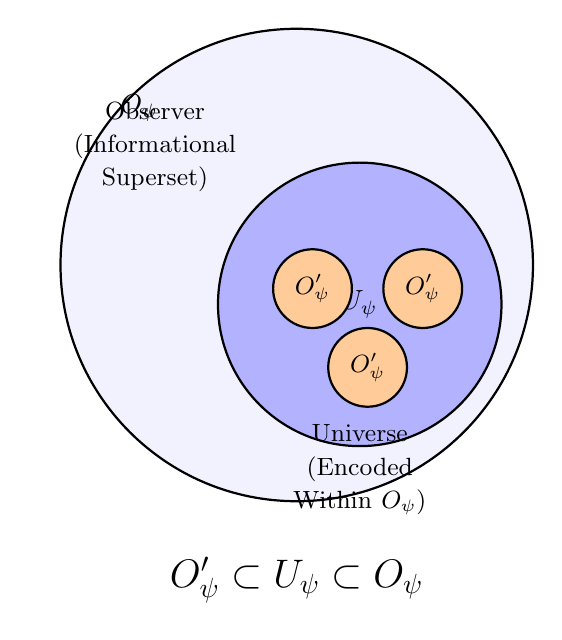
\begin{tikzpicture}
        % Observer O_\psi (Superset)
        \draw[thick, fill=blue!5] (0,0) circle (3cm);
        \node at (-2,2) {\textbf{$O_{\psi}$}};
        \node[text width=3cm, align=center] at (-1.8,1.5)
            {\small Observer\\(Informational Superset)};

        % Universe U_\psi (Encoded Subset)
        \draw[thick, fill=blue!30] (0.8,-0.5) circle (1.8cm);
        \node at (0.8,-0.5) {\textbf{$U_{\psi}$}};
        \node[text width=3cm, align=center] at (0.8,-2.6)
            {\small Universe\\(Encoded Within $O_{\psi}$)};

        % Other Observers O'_\psi
        \draw[thick, fill=orange!40] (0.2,-0.3) circle (0.5cm);
        \node at (0.2,-0.3) {\small \textbf{$O'_{\psi}$}};

        \draw[thick, fill=orange!40] (1.6,-0.3) circle (0.5cm);
        \node at (1.6,-0.3) {\small \textbf{$O'_{\psi}$}};

        \draw[thick, fill=orange!40] (0.9,-1.3) circle (0.5cm);
        \node at (0.9,-1.3) {\small \textbf{$O'_{\psi}$}};

        % Set relation
        \node at (0,-4) {\Large $O'_{\psi} \subset U_{\psi} \subset O_{\psi}$};
    \end{tikzpicture}
    \caption{Wavefunction-indexed encoding: the universe and other observers exist only as structures within the observer’s wavefunction.}
\end{figure}

This theory predicts that part of other observers always remains inaccessible to us. 


\subsection*{What motivates the focus on Spectral Complexity?}

Direct observational evidence. When we peer into the micro-cosmos, reality does not present itself as discrete, isolated digital bits;
it manifests fundamentally as continuous waves.
Spectral complexity provides the precise, continuous, and computable metric needed to bridge discrete information with the wave mechanics of actual physics.


\subsection*{Does the theory explain why the cosmic expansion rate is near-critical?}

Conditional on typical observer emergence, we are overwhelmingly likely to find ourselves situated near the peak of the microstructure count.
The expansion rate is the derivative of the lognormal - approximately zero. 

In spacetime geometry, this exact statistical spot maps directly to a near-critical expansion density ($\Omega \approx 1$).
